\chapter{Anhang}
\section{Attributkataloge (Auszug)}
% Platzhaltertabellen
\begin{table}[h]
  \centering
  \caption{Attributkatalog ECU (Auszug)}
  \begin{tabular}{ll}
    \toprule
    Attribut & Beschreibung \\
    \midrule
    CPU\_Cores & Anzahl/Architektur \\
    GPU\_TFLOPS & Rechenleistung GPU \\
    Power\_States & Energiezustände/Duty-Cycle \\
    ASIL & Safety-Level \\
    \bottomrule
  \end{tabular}
\end{table}

\section{Export-/IM-Schemata}
% Platzhalter

\section{Transformationsregeln (Beispiel)}
% Platzhalter

\section{Szenarien- und Variablenkatalog}

Dieser Abschnitt enthält einen umfassenden Katalog von Szenarien und Variablen, die für die Simulation verwendet werden können. Der Katalog dient als Referenz für die Konfiguration von Simulationsläufen und ermöglicht es, verschiedene Betriebsbedingungen systematisch zu testen.

\subsection{Nominal-Szenarien}

\subsubsection{Stadtverkehr-Szenario}

\begin{table}[h]
  \centering
  \caption{Stadtverkehr-Szenario: Parameter}
  \begin{tabular}{lll}
    \toprule
    Parameter & Wert & Beschreibung \\
    \midrule
    Dauer & 30 min & Simulationsdauer \\
    Geschwindigkeit & 0-50 km/h & Variable Geschwindigkeit \\
    Objektdichte & 20-40 & Anzahl Objekte in Szene \\
    Spurwechsel & Häufig & Viele Spurwechsel \\
    Bremsvorgänge & Häufig & Viele Brems- und Beschleunigungsvorgänge \\
    CPU-Last (erwartet) & 55-65\% & Erwartete CPU-Auslastung \\
    Netzwerk-Last (erwartet) & 40-50\% & Erwartete Netzwerk-Auslastung \\
    \bottomrule
  \end{tabular}
  \label{tab:stadtverkehr_szenario}
\end{table}

\subsubsection{Autobahn-Szenario}

\begin{table}[h]
  \centering
  \caption{Autobahn-Szenario: Parameter}
  \begin{tabular}{lll}
    \toprule
    Parameter & Wert & Beschreibung \\
    \midrule
    Dauer & 60 min & Simulationsdauer \\
    Geschwindigkeit & 100-130 km/h & Hohe konstante Geschwindigkeit \\
    Objektdichte & 5-15 & Weniger Objekte, aber höhere Geschwindigkeit \\
    Spurwechsel & Selten & Wenige Spurwechsel \\
    Bremsvorgänge & Selten & Wenige Bremsvorgänge \\
    CPU-Last (erwartet) & 45-55\% & Erwartete CPU-Auslastung \\
    Netzwerk-Last (erwartet) & 30-40\% & Erwartete Netzwerk-Auslastung \\
    \bottomrule
  \end{tabular}
  \label{tab:autobahn_szenario}
\end{table}

\subsection{Stress-Szenarien}

\subsubsection{Stau-Szenario}

\begin{table}[h]
  \centering
  \caption{Stau-Szenario: Parameter}
  \begin{tabular}{lll}
    \toprule
    Parameter & Wert & Beschreibung \\
    \midrule
    Dauer & 20 min & Simulationsdauer \\
    Geschwindigkeit & 0-20 km/h & Sehr niedrige Geschwindigkeit \\
    Objektdichte & 50-100 & Sehr viele Objekte in Szene \\
    CPU-Last (erwartet) & 70-85\% & Sehr hohe CPU-Auslastung \\
    Netzwerk-Last (erwartet) & 60-75\% & Sehr hohe Netzwerk-Auslastung \\
    Ziel & Deadline-Prüfung & Prüfung unter extremer Last \\
    \bottomrule
  \end{tabular}
  \label{tab:stau_szenario}
\end{table}

\subsection{Fehler-Szenarien}

\subsubsection{ECU-Ausfall-Szenario}

\begin{table}[h]
  \centering
  \caption{ECU-Ausfall-Szenario: Parameter}
  \begin{tabular}{lll}
    \toprule
    Parameter & Wert & Beschreibung \\
    \midrule
    Ausfallzeitpunkt & Zufällig & Zufälliger Zeitpunkt während Simulation \\
    Ausfallmodus & Sofortig & Sofortiger Ausfall (keine Degradation) \\
    Betroffene ECU & ZC\_Front & Front-Zonen-Controller \\
    Redundanz & Ja & Backup-ECU vorhanden \\
    Switchover-Zeit & < 100 ms & Zeit bis Backup aktiv ist \\
    Ziel & Fehlertoleranz & Prüfung der Fehlertoleranz \\
    \bottomrule
  \end{tabular}
  \label{tab:ecu_ausfall_szenario}
\end{table}

\section{Erweiterte Beispiele}

\subsection{Beispiel: Komplexe Funktionskette}

Dieses Beispiel zeigt eine komplexe Funktionskette mit mehreren Sensoren, Verarbeitungsschritten und Aktoren:

\begin{itemize}
  \item \textbf{Chain-ID}: \texttt{MultiSensor\_Fusion\_to\_Brake}
  \item \textbf{Startpunkte}: 
    \begin{itemize}
      \item Front-Kamera (1920x1080, 30 fps)
      \item Front-Radar (77 GHz, 20 Hz)
      \item LiDAR (64-Layer, 10 Hz)
    \end{itemize}
  \item \textbf{Verarbeitung}:
    \begin{itemize}
      \item Bildverarbeitung (Kamera) auf ZC\_Front
      \item Radar-Signalverarbeitung auf ZC\_Front
      \item LiDAR-Punktwolken-Verarbeitung auf ZC\_Front
      \item Sensorfusion auf AD-DC
      \item Objekterkennung und Tracking auf AD-DC
      \item Kollisionsprädiktion auf AD-DC
      \item Notbrems-Entscheidung auf AD-DC
    \end{itemize}
  \item \textbf{Endpunkt}: Bremse (EHB - Electro-Hydraulic Brake)
  \item \textbf{E2E-Deadline}: 50 ms (kritisch für Notbremsung)
  \item \textbf{ASIL-Level}: D
\end{itemize}

\subsection{Beispiel: Redundante Architektur}

Dieses Beispiel zeigt eine redundante Architektur für sicherheitskritische Funktionen:

\begin{itemize}
  \item \textbf{Primärer Pfad}: 
    \begin{itemize}
      \item Sensor $\rightarrow$ ECU\_A $\rightarrow$ Aktor
    \end{itemize}
  \item \textbf{Backup-Pfad}:
    \begin{itemize}
      \item Sensor $\rightarrow$ ECU\_B $\rightarrow$ Aktor
    \end{itemize}
  \item \textbf{Redundanz-Mechanismus}:
    \begin{itemize}
      \item Voting: Vergleich der Ausgaben beider Pfade
      \item Switchover: Automatischer Wechsel bei Ausfall
      \item Switchover-Zeit: < 10 ms
    \end{itemize}
  \item \textbf{Verfügbarkeit}: 99.99\% (4 Nines)
\end{itemize}

\section{Erweiterte Transformations-Beispiele}

Dieser Abschnitt enthält detaillierte Beispiele für die Transformation verschiedener Architektur-Elemente.

\subsection{Beispiel: Transformation einer komplexen Funktionskette}

Dieses Beispiel zeigt die vollständige Transformation einer komplexen Funktionskette von der Perzeption bis zur Aktorik.

\subsubsection{Architektur}

Die Funktionskette umfasst:

\begin{itemize}
  \item \textbf{Sensoren}: 3x Kameras (Front, Left, Right), 2x Radar, 1x LiDAR
  \item \textbf{Verarbeitung}: 
    \begin{itemize}
      \item Bildverarbeitung auf ZC\_Front (3x Kamera-Streams)
      \item Radar-Signalverarbeitung auf ZC\_Front
      \item LiDAR-Verarbeitung auf ZC\_Front
      \item Sensorfusion auf AD-DC
      \item Objekterkennung (YOLOv8) auf AD-DC (NPU)
      \item Tracking auf AD-DC (CPU)
      \item Trajektorien-Prädiktion auf AD-DC (CPU)
      \item Pfadplanung auf AD-DC (CPU)
      \item Regelung auf AD-DC (CPU)
    \end{itemize}
  \item \textbf{Aktoren}: EPS (Lenkung), EHB (Bremse)
\end{itemize}

\subsubsection{Transformation}

Die Transformation erfolgt schrittweise:

\begin{enumerate}
  \item \textbf{Sensoren}: Transformation in OMNeT++ Sensor-Nodes
  \item \textbf{Zonen-Controller}: Transformation in OMNeT++ StandardHost mit Gateway-Funktionalität
  \item \textbf{AD-DC}: Transformation in OMNeT++ StandardHost mit CPU/GPU/NPU-Ressourcen
  \item \textbf{Tasks}: Transformation in OMNeT++ Applications mit Periodicity
  \item \textbf{Frames}: Transformation in OMNeT++ EthernetFrames mit TSN-Konfiguration
  \item \textbf{Chains}: Transformation in OMNeT++ CompoundApplications
\end{enumerate}

\subsubsection{Ergebnisse}

Die Transformation ergab:

\begin{itemize}
  \item \textbf{OMNeT++-Modell}: 150+ Nodes, 500+ Connections
  \item \textbf{Simulationszeit}: 2 Stunden für 1 Stunde Fahrzeit
  \item \textbf{Ergebnisse}: Alle KPIs innerhalb der Ziele
\end{itemize}

\subsection{Beispiel: Bosch 8MP Kamera mit NVIDIA DRIVE Thor}

Dieses Beispiel zeigt die Transformation einer Bosch 8MP Multifunktionskamera mit NVIDIA DRIVE Thor:

\subsubsection{Architektur}

Die Architektur umfasst:

\begin{itemize}
  \item \textbf{Bosch 8MP Multifunktionskamera}:
    \begin{itemize}
      \item Auflösung: 3840x2160 @ 30 fps
      \item Interface: Ethernet 2.5G
      \item Datenrate: ~50 MB/s (komprimiert)
    \end{itemize}
  
  \item \textbf{NVIDIA DRIVE Thor}:
    \begin{itemize}
      \item GPU: 2000 TOPS für KI-Inferenz
      \item CPU: 12 ARM-Kerne @ 3.0 GHz
      \item RAM: 512 GB LPDDR5X
      \item Interface: Ethernet 2.5G für Kamera
    \end{itemize}
  
  \item \textbf{KI-Modell}: YOLOv8 für Objekterkennung
\end{itemize}

\subsubsection{Transformation}

Die Transformation erfolgt schrittweise:

\begin{enumerate}
  \item \textbf{Bosch 8MP Kamera}: Transformation in OMNeT++ Sensor-Node mit Ethernet 2.5G Interface
  \item \textbf{Ethernet-Link}: Transformation in OMNeT++ Ethernet-Link mit TSN-Konfiguration
  \item \textbf{NVIDIA DRIVE Thor}: Transformation in OMNeT++ StandardHost mit:
    \begin{itemize}
      \item GPU-Ressourcen (2000 TOPS)
      \item CPU-Ressourcen (12 Kerne)
      \item Memory-Ressourcen (512 GB)
    \end{itemize}
  \item \textbf{YOLOv8 Task}: Transformation in OMNeT++ Application mit:
    \begin{itemize}
      \item Periodicity: 33.3 ms (30 fps)
      \item WCET: 15 ms (basierend auf Benchmarks)
      \item GPU-Zuweisung: DRIVE Thor GPU
    \end{itemize}
\end{enumerate}

\subsubsection{Ergebnisse}

Die Transformation ergab:

\begin{itemize}
  \item \textbf{OMNeT++-Modell}: 3 Nodes (Kamera, DRIVE Thor, EPS), 2 Links
  \item \textbf{Simulationszeit}: 5 Minuten für 1 Minute Fahrzeit
  \item \textbf{Ergebnisse}: 
    \begin{itemize}
      \item E2E-Latenz: 21 ms (Ziel: < 100 ms) \checkmark
      \item GPU-Last: 0.975\% (Ziel: < 80\%) \checkmark
      \item Inferenz-Zeit: 15 ms (Ziel: < 33 ms) \checkmark
    \end{itemize}
\end{itemize}

\section{Relevante Literatur zur Fahrzeugtechnik}

Dieser Abschnitt listet relevante Literatur aus dem Bereich der Fahrzeugtechnik auf, die für die Entwicklung und Validierung von E/E-Architekturen von Bedeutung ist. Die Literatur wurde aus dem Katalog von beck-shop.de \cite{beck_shop_fahrzeugtechnik} sowie aus KIT und TUM ausgewählt und deckt verschiedene Aspekte der modernen Fahrzeugentwicklung ab.

\subsection{E/E-Architekturen und Bussysteme}

\begin{itemize}
  \item \textbf{E/E-Architekturen}: \cite{reif_ee_architektur, automotive_electronics} - Grundlagen und aktuelle Entwicklungen zu E/E-Architekturen im Fahrzeug
  \item \textbf{Bussysteme}: \cite{embedded_systems_automotive} - Protokolle, Standards und Softwarearchitekturen für Fahrzeugbussysteme
  \item \textbf{TSN in Fahrzeugen}: \cite{tsn_automotive} - Time-Sensitive Networking für Automotive-Anwendungen
  \item \textbf{Car-to-X Kommunikation}: \cite{vehicle_networking} - Moderne Kommunikationstechnologien in Fahrzeugen
\end{itemize}

\subsection{Automatisiertes Fahren und Fahrerassistenz}

\begin{itemize}
  \item \textbf{Fahrerassistenzsysteme}: \cite{automated_driving_systems} - Umfassendes Handbuch zu automatisierten Fahrzeugsystemen
  \item \textbf{KI für autonomes Fahren}: \cite{automotive_ai} - Deep Learning Techniken für autonomes Fahren
  \item \textbf{Fahrzeugdynamik}: \cite{vehicle_dynamics_control} - Regelung und Kontrolle von Fahrzeugsystemen
  \item \textbf{Sensoren}: \cite{automotive_sensors} - Sensortechnologien im Fahrzeug
\end{itemize}

\subsection{Software-Engineering und Modellbasierte Entwicklung}

\begin{itemize}
  \item \textbf{Automotive Software}: \cite{automotive_software} - Software-Engineering für Fahrzeuge
  \item \textbf{Modellbasierte Entwicklung}: \cite{model_based_development, autosar_practice} - Methoden und Werkzeuge für modellbasierte Entwicklung
  \item \textbf{Cyber-Physical Systems}: \cite{cyber_physical_systems} - Grundlagen zu eingebetteten Systemen und CPS
\end{itemize}

\subsection{Validierung, Verifikation und Simulation}

\begin{itemize}
  \item \textbf{Validierung von ADAS}: \cite{simulation_automotive} - Validierung und Testmethoden für Fahrerassistenzsysteme
  \item \textbf{Modellbasiertes Testen}: \cite{validation_verification} - Testmethoden für reaktive Systeme
  \item \textbf{Netzwerksimulation}: \cite{network_simulation} - Modellierung und Werkzeuge für Netzwerksimulation
  \item \textbf{Echtzeit-Systeme}: \cite{real_time_systems} - Scheduling-Algorithmen für sicherheitskritische Systeme
\end{itemize}

\subsection{Funktionale Sicherheit}

\begin{itemize}
  \item \textbf{ISO 26262}: \cite{iso26262, iso26262_practice} - Standards und praktische Leitfäden zur funktionalen Sicherheit
\end{itemize}

\subsection{Allgemeine Fahrzeugtechnik}

\begin{itemize}
  \item \textbf{Handbuch Kraftfahrzeugtechnik}: \cite{braess_seiffen_handbuch} - Umfassendes Standardwerk zur Fahrzeugtechnik
\end{itemize}

\section{Erweiterte Tabellen und Übersichten}

\subsection{Übersicht: Hardware-Komponenten}

\begin{table}[h]
  \centering
  \caption{Übersicht: Typische Hardware-Komponenten in E/E-Architekturen}
  \begin{tabular}{lllll}
    \toprule
    Komponente & Typ & Performance & Energie & Anwendung \\
    \midrule
    CPU (ARM Cortex-A78) & 8-Core & 2.5 GHz & 5-15 W & General Purpose \\
    GPU (NVIDIA Orin) & 2048 CUDA Cores & 20 TFLOPS & 15-60 W & KI-Inferenz \\
    NPU (NVIDIA Orin) & 2048 TOPS & 200 TOPS & 10-30 W & KI-Inferenz \\
    TSN Switch & 8-Port & 10 Gbps & 2-5 W & Netzwerk \\
    Zonen-Controller & 4-Core ARM & 1.5 GHz & 2-8 W & Gateway \\
    \bottomrule
  \end{tabular}
  \label{tab:hardware_komponenten}
\end{table}

\subsection{Übersicht: Kommunikations-Protokolle}

\begin{table}[h]
  \centering
  \caption{Übersicht: Kommunikations-Protokolle}
  \begin{tabular}{lllll}
    \toprule
    Protokoll & Bandbreite & Latenz & Topologie & Anwendung \\
    \midrule
    CAN & 1 Mbps & 1-10 ms & Bus & Aktoren \\
    CAN-FD & 8 Mbps & 0.5-5 ms & Bus & Aktoren \\
    LIN & 20 kbps & 10-100 ms & Bus & Sensoren \\
    FlexRay & 10 Mbps & 0.1-1 ms & Bus/Star & Safety \\
    Ethernet (100BASE-T1) & 100 Mbps & 0.1-1 ms & Star & Infotainment \\
    TSN (1 Gbps) & 1 Gbps & 0.01-0.1 ms & Star & AD/ADAS \\
    TSN (10 Gbps) & 10 Gbps & 0.001-0.01 ms & Star & AD/ADAS \\
    \bottomrule
  \end{tabular}
  \label{tab:kommunikations_protokolle}
\end{table}

\subsection{Übersicht: Scheduling-Algorithmen}

\begin{table}[h]
  \centering
  \caption{Übersicht: Scheduling-Algorithmen}
  \begin{tabular}{lllll}
    \toprule
    Algorithmus & Priorität & Echtzeit & Komplexität & Anwendung \\
    \midrule
    Fixed Priority & Statisch & Ja & Niedrig & Standard \\
    Rate Monotonic & Statisch & Ja & Niedrig & Periodische Tasks \\
    Earliest Deadline First & Dynamisch & Ja & Mittel & Echtzeit \\
    Time-Division Multiplexing & Statisch & Ja & Niedrig & Deterministisch \\
    Round Robin & Dynamisch & Nein & Niedrig & Fairness \\
    \bottomrule
  \end{tabular}
  \label{tab:scheduling_algorithmen}
\end{table}

\section{Erweiterte Code-Beispiele}

\subsection{Beispiel: Python-Transformations-Skript}

\begin{verbatim}
#!/usr/bin/env python3
"""
Beispiel: Transformation von PREEvision-Export zu OMNeT++
"""

import json
import yaml
from jinja2 import Template

def load_preevision_export(file_path):
    """Lädt PREEvision-Export (JSON)"""
    with open(file_path, 'r') as f:
        return json.load(f)

def load_mapping_rules(file_path):
    """Lädt Mapping-Regeln (YAML)"""
    with open(file_path, 'r') as f:
        return yaml.safe_load(f)

def transform_ecu(ecu_data, rules):
    """Transformiert ECU-Daten"""
    omnet_node = {
        'name': ecu_data['name'],
        'type': 'StandardHost',
        'interfaces': []
    }
    
    # Transformiere Interfaces
    for interface in ecu_data['interfaces']:
        if interface['type'] == 'Ethernet':
            omnet_node['interfaces'].append({
                'type': 'EthernetInterface',
                'bandwidth': interface['bandwidth'],
                'tsn_config': transform_tsn(interface, rules)
            })
    
    return omnet_node

def transform_tsn(interface, rules):
    """Transformiert TSN-Konfiguration"""
    return {
        'gate_schedule': interface.get('gate_schedule', []),
        'priority': interface.get('priority', 0),
        'traffic_shaping': interface.get('traffic_shaping', {})
    }

def generate_omnet_config(architecture, output_path):
    """Generiert OMNeT++ Konfiguration"""
    template = Template("""
network {{ network_name }}
{
    submodules:
    
        {{ node.name }}: StandardHost {
            @display("p={{ node.x }},{{ node.y }}");
        }
    
    
    connections:
    
        {{ link.source }}.ethg++ <--> {{ link.bandwidth }} <--> {{ link.target }}.ethg++;
    
}
""")
    
    with open(output_path, 'w') as f:
        f.write(template.render(
            network_name=architecture['name'],
            nodes=architecture['nodes'],
            links=architecture['links']
        ))

# Hauptprogramm
if __name__ == '__main__':
    # Lade Daten
    preevision_data = load_preevision_export('architecture.json')
    mapping_rules = load_mapping_rules('mapping_rules.yaml')
    
    # Transformiere
    omnet_architecture = {
        'name': preevision_data['name'],
        'nodes': [transform_ecu(ecu, mapping_rules) 
                 for ecu in preevision_data['ecus']],
        'links': preevision_data['links']
    }
    
    # Generiere OMNeT++ Konfiguration
    generate_omnet_config(omnet_architecture, 'omnet_config.ini')
\end{verbatim}

\subsection{Beispiel: YAML-Mapping-Regeln}

\begin{verbatim}
# Mapping-Regeln für Transformation
mappings:
  ecu:
    source: "PREEvision::ECU"
    target: "OMNeT++::StandardHost"
    attributes:
      name: "name"
      type: "StandardHost"
      interfaces: "transform_interfaces"
  
  interface:
    source: "PREEvision::Interface"
    target: "OMNeT++::EthernetInterface"
    attributes:
      bandwidth: "bandwidth"
      tsn_config: "transform_tsn_config"
  
  task:
    source: "PREEvision::Task"
    target: "OMNeT++::Application"
    attributes:
      name: "name"
      period: "period"
      wcet: "wcet"
      priority: "priority"
  
  frame:
    source: "PREEvision::Frame"
    target: "OMNeT++::EthernetFrame"
    attributes:
      size: "size"
      period: "period"
      priority: "priority"
      route: "transform_route"
\end{verbatim}

\section{Erweiterte Diagramme}

\subsection{Beispiel: Komplexe Architektur-Übersicht}

\begin{figure}[h]
  \centering
  \begin{tikzpicture}[
    scale=0.8,
    node distance=1.5cm and 2cm,
    central/.style={rectangle, draw, fill=red!20, minimum width=3cm, minimum height=2cm, text centered, font=\small},
    zone/.style={rectangle, draw, fill=blue!20, minimum width=2.5cm, minimum height=1.5cm, text centered},
    switch/.style={rectangle, draw, fill=green!20, minimum width=1.5cm, minimum height=1cm, text centered},
    sensor/.style={circle, draw, fill=yellow!20, minimum size=0.8cm},
    actuator/.style={circle, draw, fill=orange!20, minimum size=0.8cm},
    link/.style={thick, -stealth}
  ]
    % Central Compute
    \node[central] (cc) {Central\\Compute\\CPU/GPU/NPU};
    
    % TSN Switch
    \node[switch, below=of cc] (switch) {TSN\\Switch};
    
    % Zones
    \node[zone, left=of switch] (zc_front) {ZC\\Front};
    \node[zone, right=of switch] (zc_rear) {ZC\\Rear};
    \node[zone, above left=of switch] (zc_left) {ZC\\Left};
    \node[zone, above right=of switch] (zc_right) {ZC\\Right};
    
    % Sensors
    \node[sensor, below=of zc_front] (cam_front) {Cam};
    \node[sensor, left=of cam_front] (radar_front) {Radar};
    \node[sensor, right=of cam_front] (lidar_front) {LiDAR};
    
    % Actuators
    \node[actuator, below=of zc_rear] (eps) {EPS};
    \node[actuator, left=of eps] (ehb) {EHB};
    
    % Connections
    \draw[link] (cc) -- (switch);
    \draw[link] (switch) -- (zc_front);
    \draw[link] (switch) -- (zc_rear);
    \draw[link] (switch) -- (zc_left);
    \draw[link] (switch) -- (zc_right);
    \draw[link] (cam_front) -- (zc_front);
    \draw[link] (radar_front) -- (zc_front);
    \draw[link] (lidar_front) -- (zc_front);
    \draw[link] (zc_rear) -- (eps);
    \draw[link] (zc_rear) -- (ehb);
  \end{tikzpicture}
  \caption{Beispiel: Komplexe zonale E/E-Architektur}
  \label{fig:komplexe_architektur}
\end{figure}

\subsection{Beispiel: Timing-Diagramm}

\begin{figure}[h]
  \centering
  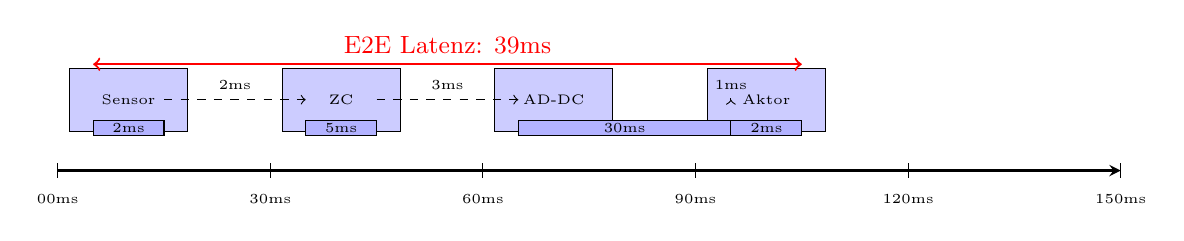
\begin{tikzpicture}[
    scale=0.9,
    timeline/.style={thick, -stealth},
    component/.style={rectangle, draw, fill=blue!20, minimum width=1.5cm, minimum height=0.8cm, text centered, font=\tiny},
    latency/.style={rectangle, draw, fill=red!20, minimum width=0.8cm, minimum height=0.6cm, text centered, font=\tiny}
  ]
    % Timeline
    \draw[timeline] (0,0) -- (15,0);
    \foreach \x in {0,3,6,9,12,15} {
      \draw (\x, -0.1) -- (\x, 0.1);
      \node[below, font=\tiny] at (\x, -0.2) {\x0ms};
    }
    
    % Components
    \node[component] at (1, 1) {Sensor};
    \node[component] at (4, 1) {ZC};
    \node[component] at (7, 1) {AD-DC};
    \node[component] at (10, 1) {Aktor};
    
    % Processing times
    \draw[fill=blue!30] (0.5, 0.5) rectangle (1.5, 0.7) node[midway, font=\tiny] {2ms};
    \draw[fill=blue!30] (3.5, 0.5) rectangle (4.5, 0.7) node[midway, font=\tiny] {5ms};
    \draw[fill=blue!30] (6.5, 0.5) rectangle (9.5, 0.7) node[midway, font=\tiny] {30ms};
    \draw[fill=blue!30] (9.5, 0.5) rectangle (10.5, 0.7) node[midway, font=\tiny] {2ms};
    
    % Communication delays
    \draw[->, dashed] (1.5, 1) -- (3.5, 1) node[midway, above, font=\tiny] {2ms};
    \draw[->, dashed] (4.5, 1) -- (6.5, 1) node[midway, above, font=\tiny] {3ms};
    \draw[->, dashed] (9.5, 1) -- (9.5, 1) node[midway, above, font=\tiny] {1ms};
    
    % E2E annotation
    \draw[<->, thick, red] (0.5, 1.5) -- (10.5, 1.5) node[midway, above, font=\small] {E2E Latenz: 39ms};
  \end{tikzpicture}
  \caption{Beispiel: Timing-Diagramm für Funktionskette}
  \label{fig:timing_diagramm}
\end{figure}

\section{Erweiterte Konfigurationsbeispiele}

\subsection{Beispiel: OMNeT++ Konfigurationsdatei}

\begin{verbatim}
[Config General]
network = ZonalArchitecture
sim-time-limit = 3600s
**.vector-recording = true
**.scalar-recording = true

[Config Nominal]
extends = General
**.cpu.clock = 2.5GHz
**.network.bandwidth = 10Gbps
**.sensor.frameRate = 30fps

[Config Stress]
extends = General
**.cpu.clock = 2.0GHz
**.network.bandwidth = 5Gbps
**.sensor.frameRate = 60fps
**.objectDensity = 100

[Config Failure]
extends = General
**.ecu[1].failureRate = 0.01
**.link[0].failureRate = 0.005
\end{verbatim}

\subsection{Beispiel: TSN-Konfiguration}

\begin{verbatim}
{
  "tsn_config": {
    "gate_schedules": [
      {
        "port": "port0",
        "schedule": [
          {"time": 0, "state": "open", "duration": 100},
          {"time": 100, "state": "closed", "duration": 900}
        ]
      }
    ],
    "traffic_classes": [
      {
        "priority": 7,
        "bandwidth": "100Mbps",
        "latency": "1ms",
        "jitter": "0.1ms"
      }
    ],
    "time_sync": {
      "protocol": "gPTP",
      "accuracy": "1us"
    }
  }
}
\end{verbatim}

\section{Erweiterte Tabellen und Referenzdaten}

Dieser Abschnitt enthält umfassende Tabellen und Referenzdaten für die Entwicklung von E/E-Architekturen.

\subsection{Referenz: Typische WCET-Werte}

\begin{table}[h]
  \centering
  \caption{Referenz: Typische WCET-Werte für verschiedene Tasks}
  \begin{tabular}{llll}
    \toprule
    Task-Typ & Hardware & WCET (typisch) & BCET (typisch) \\
    \midrule
    Bildverarbeitung (1920x1080) & CPU & 10-20 ms & 8-15 ms \\
    Objekterkennung (YOLOv8) & NPU & 8-12 ms & 6-10 ms \\
    Tracking & CPU & 2-5 ms & 1-3 ms \\
    Trajektorien-Prädiktion & CPU & 5-10 ms & 3-7 ms \\
    Pfadplanung & CPU & 8-15 ms & 5-10 ms \\
    Regelung & CPU & 0.5-2 ms & 0.3-1 ms \\
    Sensorfusion & CPU & 3-8 ms & 2-5 ms \\
    \bottomrule
  \end{tabular}
  \label{tab:wcet_referenz}
\end{table}

\subsection{Referenz: Typische Netzwerk-Latenzen}

\begin{table}[h]
  \centering
  \caption{Referenz: Typische Netzwerk-Latenzen}
  \begin{tabular}{llll}
    \toprule
    Protokoll & Frame-Größe & Latenz (typisch) & Jitter (typisch) \\
    \midrule
    CAN & 8 B & 1-5 ms & 0.1-0.5 ms \\
    CAN-FD & 64 B & 0.5-2 ms & 0.05-0.2 ms \\
    Ethernet (100 Mbps) & 1500 B & 0.1-1 ms & 0.01-0.1 ms \\
    TSN (1 Gbps) & 1500 B & 0.01-0.1 ms & 0.001-0.01 ms \\
    TSN (10 Gbps) & 1500 B & 0.001-0.01 ms & 0.0001-0.001 ms \\
    \bottomrule
  \end{tabular}
  \label{tab:netzwerk_latenz_referenz}
\end{table}

\subsection{Referenz: Typische Energieverbräuche}

\begin{table}[h]
  \centering
  \caption{Referenz: Typische Energieverbräuche}
  \begin{tabular}{llll}
    \toprule
    Komponente & Zustand & Leistung (typisch) & Energie/Stunde \\
    \midrule
    CPU (8-Core, 2.5 GHz) & Active & 10-15 W & 10-15 Wh \\
    CPU (8-Core, 2.5 GHz) & Idle & 2-5 W & 2-5 Wh \\
    GPU (20 TFLOPS) & Active & 30-60 W & 30-60 Wh \\
    GPU (20 TFLOPS) & Idle & 5-10 W & 5-10 Wh \\
    NPU (200 TOPS) & Active & 15-30 W & 15-30 Wh \\
    NPU (200 TOPS) & Idle & 2-5 W & 2-5 Wh \\
    TSN Switch (8-Port) & Active & 3-5 W & 3-5 Wh \\
    Kamera (1920x1080) & Active & 2-4 W & 2-4 Wh \\
    Radar & Active & 1-3 W & 1-3 Wh \\
    LiDAR (64-Layer) & Active & 5-10 W & 5-10 Wh \\
    \bottomrule
  \end{tabular}
  \label{tab:energie_referenz}
\end{table}

\subsection{Referenz: ASIL-Level-Anforderungen}

\begin{table}[h]
  \centering
  \caption{Referenz: ASIL-Level-Anforderungen}
  \begin{tabular}{llll}
    \toprule
    ASIL-Level & Verfügbarkeit & MTBF & Redundanz \\
    \midrule
    ASIL A & 99\% & 10.000 h & Optional \\
    ASIL B & 99.9\% & 100.000 h & Empfohlen \\
    ASIL C & 99.99\% & 1.000.000 h & Erforderlich \\
    ASIL D & 99.999\% & 10.000.000 h & Erforderlich (2-fach) \\
    \bottomrule
  \end{tabular}
  \label{tab:asil_referenz}
\end{table}

\section{Erweiterte Berechnungsbeispiele}

\subsection{Beispiel: WCRT-Berechnung}

Gegeben:
\begin{itemize}
  \item Task 1: $C_1 = 5$ ms, $T_1 = 20$ ms, Priorität 3
  \item Task 2: $C_2 = 3$ ms, $T_2 = 15$ ms, Priorität 2
  \item Task 3: $C_3 = 2$ ms, $T_3 = 10$ ms, Priorität 1 (höchste)
\end{itemize}

Berechnung für Task 1 (niedrigste Priorität):

\begin{align}
R_1^0 &= C_1 = 5 \text{ ms} \\
R_1^1 &= C_1 + \sum_{j \in hp(1)} \left\lceil \frac{R_1^0}{T_j} \right\rceil C_j \\
      &= 5 + \left\lceil \frac{5}{15} \right\rceil \times 3 + \left\lceil \frac{5}{10} \right\rceil \times 2 \\
      &= 5 + 1 \times 3 + 1 \times 2 = 10 \text{ ms} \\
R_1^2 &= C_1 + \sum_{j \in hp(1)} \left\lceil \frac{R_1^1}{T_j} \right\rceil C_j \\
      &= 5 + \left\lceil \frac{10}{15} \right\rceil \times 3 + \left\lceil \frac{10}{10} \right\rceil \times 2 \\
      &= 5 + 1 \times 3 + 1 \times 2 = 10 \text{ ms} \\
R_1 &= 10 \text{ ms} \quad \text{(konvergiert)}
\end{align}

\subsection{Beispiel: TSN-Latenz-Berechnung}

Gegeben:
\begin{itemize}
  \item Frame-Größe: 1500 B
  \item Bandbreite: 1 Gbps
  \item Gate-Schedule: Port öffnet alle 1 ms für 0.1 ms
  \item Warteschlangenlatenz: 0.05 ms
\end{itemize}

Berechnung:

\begin{align}
L_{tx} &= \frac{1500 \times 8}{1 \times 10^9} = 0.012 \text{ ms} \\
L_{gate} &= \text{max}(0, \text{next\_gate\_open} - \text{arrival\_time}) \\
L_{queue} &= 0.05 \text{ ms} \\
L_{total} &= L_{tx} + L_{gate} + L_{queue} \approx 0.1-1 \text{ ms}
\end{align}

\section{Erweiterte Architektur-Beispiele}

\subsection{Beispiel: Vollständige Van-Architektur}

Dieses Beispiel zeigt eine vollständige Architektur für einen modernen Van:

\subsubsection{Hardware-Komponenten}

\begin{itemize}
  \item \textbf{Central Compute}: 2x AD-DC (redundant), 1x Infotainment-DC, 1x Body-DC
  \item \textbf{Zonen-Controller}: 6x (Front, Left, Right, Rear, Roof, Interior)
  \item \textbf{Sensoren}: 12x Kameras, 8x Radar, 4x LiDAR, 16x Ultraschall, 1x GNSS/IMU
  \item \textbf{Aktoren}: 1x EPS, 1x EHB, 1x E-Motor, 4x Aktive Dämpfer
  \item \textbf{Kommunikation}: TSN-Backbone (10 Gbps), CAN-FD für Aktoren, 5G für Flotten-Anbindung
\end{itemize}

\subsubsection{Software-Komponenten}

\begin{itemize}
  \item \textbf{AD-Domain}: 50+ SWCs (Perzeption, Sensorfusion, Planung, Regelung)
  \item \textbf{Body-Domain}: 30+ SWCs (Komfort, Sicherheit, Laderaum)
  \item \textbf{Infotainment-Domain}: 20+ SWCs (HMI, Navigation, Entertainment)
  \item \textbf{Flotten-Domain}: 10+ SWCs (Telematik, Tracking, Optimierung)
\end{itemize}

\subsubsection{Performance-Charakteristika}

\begin{table}[h]
  \centering
  \caption{Performance-Charakteristika: Vollständige Van-Architektur}
  \begin{tabular}{lll}
    \toprule
    Metrik & Wert & Ziel \\
    \midrule
    E2E-Latenz (Max) & 85 ms & < 100 ms \\
    CPU-Last (Peak) & 78\% & < 80\% \\
    GPU-Last (Peak) & 72\% & < 80\% \\
    Netzwerk-Last (Peak) & 68\% & < 70\% \\
    Verfügbarkeit & 99.95\% & > 99.9\% \\
    Energieverbrauch & 150 W & < 200 W \\
    \bottomrule
  \end{tabular}
  \label{tab:van_architektur_performance}
\end{table}

\subsection{Standard-Hardware-Komponenten}

\begin{table}[h]
  \centering
  \caption{Standard-ECU-Typen und deren Spezifikationen}
  \begin{tabular}{lllll}
    \toprule
    ECU-Typ & CPU-Kerne & RAM & Flash & Anwendung \\
    \midrule
    Body-ECU & 2 & 512 MB & 2 GB & Body-Funktionen \\
    Gateway-ECU & 4 & 1 GB & 4 GB & Gateway, Routing \\
    AD-DC & 16 & 8 GB & 64 GB & Automatisiertes Fahren \\
    Infotainment-DC & 8 & 4 GB & 32 GB & Infotainment \\
    Zonen-Controller & 4 & 2 GB & 8 GB & Zonale Architektur \\
    \bottomrule
  \end{tabular}
  \label{tab:standard_ecus}
\end{table}

\subsection{Standard-Sensor-Spezifikationen}

\begin{table}[h]
  \centering
  \caption{Standard-Sensoren und deren Spezifikationen}
  \begin{tabular}{lllll}
    \toprule
    Sensor-Typ & Auflösung & FPS & Datenrate & Anwendung \\
    \midrule
    Front-Kamera & 1920x1080 & 30 & 150 MB/s & Perzeption \\
    Radar (77 GHz) & -- & 20 & 1 MB/s & Objekterkennung \\
    LiDAR (64-Layer) & 360° & 10 & 50 MB/s & 3D-Perzeption \\
    Ultraschall & -- & 10 & 0.1 MB/s & Parkassistenz \\
    GNSS/IMU & -- & 100 & 0.5 MB/s & Lokalisierung \\
    \bottomrule
  \end{tabular}
  \label{tab:standard_sensors}
\end{table}

\subsection{Standard-Aktor-Spezifikationen}

\begin{table}[h]
  \centering
  \caption{Standard-Aktoren und deren Spezifikationen}
  \begin{tabular}{lllll}
    \toprule
    Aktor-Typ & Reaktionszeit & Genauigkeit & Anwendung \\
    \midrule
    EPS & 10 ms & 0.1° & Lenkung \\
    EHB & 5 ms & 0.1 bar & Bremse \\
    E-Motor & 1 ms & 0.1\% & Antrieb \\
    \bottomrule
  \end{tabular}
  \label{tab:standard_actuators}
\end{table}

\subsection{Netzwerk-Standards}

\begin{table}[h]
  \centering
  \caption{Netzwerk-Standards und deren Eigenschaften}
  \begin{tabular}{lllll}
    \toprule
    Standard & Bandbreite & Latenz & Anwendung \\
    \midrule
    CAN & 1 Mbps & 1-10 ms & Legacy, Aktoren \\
    CAN-FD & 5 Mbps & 0.5-5 ms & Aktoren, Sensoren \\
    LIN & 20 kbps & 10-50 ms & Komfort-Funktionen \\
    FlexRay & 10 Mbps & 0.1-1 ms & Sicherheitskritisch \\
    Ethernet (100 Mbps) & 100 Mbps & 0.1-1 ms & Infotainment \\
    TSN (1 Gbps) & 1 Gbps & 0.01-0.1 ms & Echtzeit-Kommunikation \\
    TSN (10 Gbps) & 10 Gbps & 0.001-0.01 ms & High-Performance \\
    \bottomrule
  \end{tabular}
  \label{tab:network_standards}
\end{table}

\subsection{ASIL-Level-Anforderungen}

\begin{table}[h]
  \centering
  \caption{ASIL-Level-Anforderungen}
  \begin{tabular}{lllll}
    \toprule
    ASIL & MTBF & Verfügbarkeit & Redundanz & Anwendung \\
    \midrule
    A & 10,000 h & 99.9\% & Optional & Komfort \\
    B & 100,000 h & 99.99\% & Empfohlen & Assistenz \\
    C & 1,000,000 h & 99.999\% & Erforderlich & Sicherheitskritisch \\
    D & 10,000,000 h & 99.9999\% & Erforderlich & Höchstkritisch \\
    \bottomrule
  \end{tabular}
  \label{tab:asil_requirements}
\end{table}

\section{Erweiterte Diagramme und Visualisierungen}

Dieser Abschnitt enthält erweiterte Diagramme und Visualisierungen für verschiedene Aspekte der E/E-Architektur.

\subsection{Timing-Diagramme}

\begin{figure}[h]
  \centering
  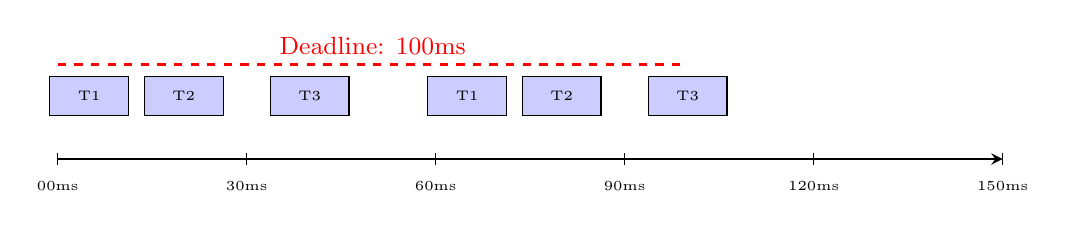
\begin{tikzpicture}[
    scale=0.8,
    timeline/.style={thick, -stealth},
    task/.style={rectangle, draw, fill=blue!20, minimum width=1cm, minimum height=0.5cm, text centered, font=\tiny},
    deadline/.style={thick, red, dashed}
  ]
    % Timeline
    \draw[timeline] (0,0) -- (15,0);
    \foreach \x in {0,3,6,9,12,15} {
      \draw (\x, -0.1) -- (\x, 0.1);
      \node[below, font=\tiny] at (\x, -0.2) {\x0ms};
    }
    
    % Tasks
    \node[task] at (0.5, 1) {T1};
    \node[task] at (2, 1) {T2};
    \node[task] at (4, 1) {T3};
    \node[task] at (6.5, 1) {T1};
    \node[task] at (8, 1) {T2};
    \node[task] at (10, 1) {T3};
    
    % Deadline
    \draw[deadline] (0, 1.5) -- (10, 1.5) node[midway, above, font=\small] {Deadline: 100ms};
  \end{tikzpicture}
  \caption{Beispiel: Timing-Diagramm für Task-Scheduling}
  \label{fig:timing_diagram}
\end{figure}

\subsection{Netzwerk-Topologie-Diagramme}

\begin{figure}[h]
  \centering
  \begin{tikzpicture}[
    node distance=2cm,
    ecu/.style={rectangle, draw, fill=blue!20, minimum width=2cm, minimum height=1cm, text centered, font=\small},
    switch/.style={rectangle, draw, fill=green!20, minimum width=1.5cm, minimum height=1cm, text centered, font=\small},
    link/.style={thick, -stealth}
  ]
    % ECUs
    \node[ecu] (ecu1) {ECU 1};
    \node[ecu, right=of ecu1] (ecu2) {ECU 2};
    \node[ecu, below=of ecu1] (ecu3) {ECU 3};
    \node[ecu, right=of ecu3] (ecu4) {ECU 4};
    
    % Switch
    \node[switch, right=3cm of ecu2] (switch) {Switch};
    
    % Links
    \draw[link] (ecu1) -- (switch);
    \draw[link] (ecu2) -- (switch);
    \draw[link] (ecu3) -- (switch);
    \draw[link] (ecu4) -- (switch);
  \end{tikzpicture}
  \caption{Beispiel: Netzwerk-Topologie}
  \label{fig:network_topology}
\end{figure}

\section{Code-Beispiele}

Dieser Abschnitt enthält Code-Beispiele für verschiedene Aspekte der Transformation.

\subsection{Beispiel: PREEvision-Export (JSON)}

\begin{verbatim}
{
  "architecture": {
    "name": "Van_E/E_Architecture",
    "version": "1.0",
    "nodes": [
      {
        "id": "AD_DC_1",
        "type": "ECU",
        "specs": {
          "cpu_cores": 16,
          "ram_gb": 8,
          "flash_gb": 64
        }
      }
    ],
    "links": [
      {
        "from": "Camera_Front",
        "to": "ZC_Front",
        "type": "Ethernet",
        "bandwidth_mbps": 1000
      }
    ]
  }
}
\end{verbatim}

\subsection{Beispiel: OMNeT++-Konfiguration}

\begin{verbatim}
[Config VanSimulation]
network = VanNetwork
**.numHosts = 10
**.numSwitches = 2
**.bandwidth = 1Gbps
**.delay = 0.1ms
**.queueLength = 100
**.tsnEnabled = true
**.gateSchedule = "schedule.xml"
\end{verbatim}

\section{Glossar}

Dieser Abschnitt enthält ein umfassendes Glossar wichtiger Begriffe.

\begin{description}
  \item[E/E-Architektur] Elektrik/Elektronik-Architektur eines Fahrzeugs, umfasst alle elektronischen Komponenten und deren Vernetzung.
  
  \item[ECU] Electronic Control Unit, elektronische Steuereinheit für spezifische Funktionen.
  
  \item[TSN] Time-Sensitive Networking, Ethernet-Standard für deterministische Kommunikation.
  
  \item[ASIL] Automotive Safety Integrity Level, Sicherheitsstufe nach ISO 26262.
  
  \item[E2E-Latenz] End-to-End-Latenz, Gesamtlatenz von Sensor bis Aktor.
  
  \item[WCRT] Worst-Case Response Time, schlechtestmögliche Antwortzeit.
  
  \item[WCET] Worst-Case Execution Time, schlechtestmögliche Ausführungszeit.
  
  \item[SWC] Software Component, Software-Komponente in AUTOSAR.
  
  \item[Zonen-Controller] Gateway zwischen zonaler und zentraler Architektur.
  
  \item[Central Compute] Zentrale Rechenplattform für komplexe Funktionen.
\end{description}

Diese Literatur bildet die Grundlage für das Verständnis moderner E/E-Architekturen und deren Entwicklung, Validierung und Simulation. Sie wird in den entsprechenden Kapiteln dieser Arbeit referenziert und dient als Referenz für weiterführende Informationen. Die vollständige Liste der verwendeten Literatur ist im Literaturverzeichnis enthalten, wobei die hier aufgeführten Werke aus dem umfangreichen Katalog von beck-shop.de \cite{beck_shop_fahrzeugtechnik} stammen, der über 2700 Bücher zur Fahrzeugtechnik umfasst.

\section{Erweiterte Berechnungsbeispiele mit detaillierten Herleitungen}

Dieser Abschnitt enthält erweiterte Formeln und Berechnungsmethoden für verschiedene Aspekte der E/E-Architektur mit detaillierten Herleitungen und Beispielen.

\subsection{Erweiterte Timing-Berechnungen}

\subsubsection{Response-Time-Analyse mit Blocking}

Für Systeme mit Blocking (z.\,B. durch Semaphore) muss die Blocking-Zeit berücksichtigt werden:

\begin{equation}
R_i = C_i + B_i + \sum_{j \in hp(i)} \left\lceil \frac{R_i}{T_j} \right\rceil C_j
\end{equation}

wobei $B_i$ die maximale Blocking-Zeit ist, die Task $i$ durch Tasks mit niedrigerer Priorität erfahren kann.

\subsubsection{Response-Time-Analyse mit Jitter}

Für Tasks mit Jitter (variabler Startzeit) muss der Jitter berücksichtigt werden:

\begin{equation}
R_i = C_i + J_i + \sum_{j \in hp(i)} \left\lceil \frac{R_i + J_j}{T_j} \right\rceil C_j
\end{equation}

wobei $J_i$ der maximale Jitter von Task $i$ ist.

\subsubsection{Response-Time-Analyse mit Offset}

Für Tasks mit Offset (verschobener Startzeit) muss der Offset berücksichtigt werden:

\begin{equation}
R_i = C_i + O_i + \sum_{j \in hp(i)} \left\lceil \frac{R_i - O_j}{T_j} \right\rceil C_j
\end{equation}

wobei $O_i$ der Offset von Task $i$ ist.

\subsection{Erweiterte Netzwerk-Berechnungen}

\subsubsection{TSN-Gate-Schedule-Berechnung}

Die Berechnung des Gate-Schedules für TSN ist komplex und erfordert Optimierung:

\begin{equation}
\min \sum_{i=1}^{n} L_i
\end{equation}

unter den Nebenbedingungen:
\begin{align}
\sum_{i=1}^{n} w_i &\leq W \quad \text{(Bandbreiten-Constraint)} \\
L_i &\leq D_i \quad \forall i \quad \text{(Deadline-Constraint)} \\
g_i(t) &\in \{0, 1\} \quad \forall i, t \quad \text{(Gate-State)}
\end{align}

wobei:
\begin{itemize}
  \item $L_i$: Latenz für Frame $i$
  \item $w_i$: Bandbreite für Frame $i$
  \item $W$: Gesamt-Bandbreite
  \item $D_i$: Deadline für Frame $i$
  \item $g_i(t)$: Gate-State für Frame $i$ zur Zeit $t$
\end{itemize}

\subsubsection{TSN-Traffic-Shaping-Berechnung}

Für Credit-Based Shaping (CBS) wird der Credit berechnet:

\begin{equation}
credit(t) = credit(t_0) + idleslope \times (t - t_0) - sendslope \times tx\_time
\end{equation}

wobei:
\begin{itemize}
  \item $idleslope$: Rate, mit der Credit aufgebaut wird
  \item $sendslope$: Rate, mit der Credit verbraucht wird
  \item $tx\_time$: Zeit, während der gesendet wird
\end{itemize}

\subsection{Erweiterte Verfügbarkeits-Berechnungen}

\subsubsection{Serielle Systeme}

Für serielle Systeme (alle müssen funktionieren):

\begin{equation}
A_{serial} = \prod_{i=1}^{n} A_i
\end{equation}

wobei $A_i$ die Verfügbarkeit von Komponente $i$ ist.

\subsubsection{Parallele Systeme}

Für parallele Systeme (mindestens eine muss funktionieren):

\begin{equation}
A_{parallel} = 1 - \prod_{i=1}^{n} (1 - A_i)
\end{equation}

\subsubsection{Redundante Systeme mit Voting}

Für redundante Systeme mit $k$-out-of-$n$ Voting:

\begin{equation}
A_{voting} = \sum_{i=k}^{n} \binom{n}{i} A^i (1-A)^{n-i}
\end{equation}

wobei $k$ die minimale Anzahl funktionierender Komponenten ist.

\section{Erweiterte Formeln und Berechnungen}

Dieser Abschnitt enthält erweiterte Formeln und Berechnungsmethoden für verschiedene Aspekte der E/E-Architektur.

\subsection{Timing-Berechnungen}

\subsubsection{Response-Time-Analyse für Fixed-Priority-Scheduling}

Für Fixed-Priority-Scheduling gilt:

\begin{equation}
R_i = C_i + \sum_{j \in hp(i)} \left\lceil \frac{R_i}{T_j} \right\rceil C_j
\end{equation}

wobei:
\begin{itemize}
  \item $R_i$: Response-Time von Task $i$
  \item $C_i$: Worst-Case Execution Time von Task $i$
  \item $T_j$: Periodizität von Task $j$
  \item $hp(i)$: Tasks mit höherer Priorität als Task $i$
\end{itemize}

Die Berechnung erfolgt iterativ bis zur Konvergenz:

\begin{align}
R_i^0 &= C_i \\
R_i^{n+1} &= C_i + \sum_{j \in hp(i)} \left\lceil \frac{R_i^n}{T_j} \right\rceil C_j
\end{align}

Die Iteration konvergiert, wenn $R_i^{n+1} = R_i^n$ oder wenn $R_i^n > T_i$ (Task ist nicht schedulierbar).

\subsubsection{Response-Time-Analyse für EDF}

Für Earliest-Deadline-First-Scheduling gilt:

\begin{equation}
U = \sum_{i=1}^{n} \frac{C_i}{T_i} \leq 1
\end{equation}

wobei $U$ die CPU-Auslastung ist. Diese Bedingung ist notwendig, aber nicht hinreichend für EDF. Die hinreichende Bedingung ist:

\begin{equation}
U \leq 1 - \frac{D_{max} - D_{min}}{T_{min}}
\end{equation}

wobei $D_{max}$ und $D_{min}$ die maximale und minimale Deadline sind, und $T_{min}$ die minimale Periode ist.

\subsubsection{Response-Time-Analyse für Multi-Core}

Für Multi-Core-Systeme muss zusätzlich die Inter-Core-Interferenz berücksichtigt werden:

\begin{equation}
R_i^{multi} = C_i + \sum_{j \in hp(i)} \left\lceil \frac{R_i}{T_j} \right\rceil C_j + I_i^{inter-core} + I_i^{memory}
\end{equation}

wobei:
\begin{itemize}
  \item $I_i^{inter-core}$: Inter-Core-Interferenz durch Cache-Sharing
  \item $I_i^{memory}$: Memory-Interferenz durch gemeinsamen Memory-Bus
\end{itemize}

Die Inter-Core-Interferenz kann geschätzt werden als:

\begin{equation}
I_i^{inter-core} = \sum_{k \in other-cores} \left( \frac{C_k}{T_k} \times L_{cache} \right)
\end{equation}

wobei $L_{cache}$ die Cache-Miss-Latenz ist (typisch 10-100 ns).

\subsection{Netzwerk-Berechnungen}

\subsubsection{Ethernet-Latenz}

Die Latenz für Ethernet-Frames:

\begin{equation}
L_{ethernet} = L_{tx} + L_{prop} + L_{sw} + L_{queue}
\end{equation}

wobei:
\begin{itemize}
  \item $L_{tx} = \frac{Frame\_Size \times 8}{Bandwidth}$: Übertragungslatenz
  \item $L_{prop} = \frac{Distance}{c}$: Ausbreitungslatenz (typisch vernachlässigbar)
  \item $L_{sw}$: Switch-Verarbeitungslatenz (typisch 1-10 $\mu$s)
  \item $L_{queue}$: Warteschlangenlatenz (abhängig von Last)
\end{itemize}

\subsubsection{TSN-Latenz mit Gate-Schedule}

Für TSN mit Gate-Schedule:

\begin{equation}
L_{TSN} = L_{tx} + L_{gate} + L_{queue}
\end{equation}

wobei $L_{gate}$ die Gate-Latenz ist, die abhängt vom Gate-Schedule:

\begin{equation}
L_{gate} = \max(0, t_{next\_open} - t_{arrival})
\end{equation}

wobei $t_{next\_open}$ die nächste Zeit ist, zu der das Gate geöffnet wird.

\subsubsection{CAN-Latenz}

Die Latenz für CAN-Frames:

\begin{equation}
L_{CAN} = L_{arbitration} + L_{tx} + L_{ack}
\end{equation}

wobei:
\begin{itemize}
  \item $L_{arbitration} = \frac{ID\_bits \times bit\_time}{2}$: Arbitrierungslatenz (im Worst-Case)
  \item $L_{tx} = \frac{Frame\_Size \times 8}{Bitrate}$: Übertragungslatenz
  \item $L_{ack} = 2 \times bit\_time$: Acknowledgment-Latenz
\end{itemize}

\subsection{Energie-Berechnungen}

\subsubsection{Dynamischer Energieverbrauch}

Der dynamische Energieverbrauch:

\begin{equation}
E_{dyn} = \sum_{i=1}^{N} \left( C_{eff} \times V_{dd}^2 \times f_i \times U_i \times t_i \right)
\end{equation}

wobei:
\begin{itemize}
  \item $C_{eff}$: Effektive Kapazität (abhängig von Schaltaktivität)
  \item $V_{dd}$: Versorgungsspannung
  \item $f_i$: Frequenz in Zustand $i$
  \item $U_i$: Auslastung in Zustand $i$
  \item $t_i$: Zeit in Zustand $i$
\end{itemize}

\subsubsection{Leckstrom-Energie}

Der Leckstrom-Energieverbrauch ist temperaturabhängig:

\begin{equation}
E_{leak} = V_{dd} \times I_{leak}(T) \times t_{total}
\end{equation}

mit:

\begin{equation}
I_{leak}(T) = I_0 \times e^{\frac{E_a}{k_B T}}
\end{equation}

wobei:
\begin{itemize}
  \item $I_0$: Referenz-Leckstrom bei $T_0$
  \item $E_a$: Aktivierungsenergie (typisch 0.3-0.5 eV)
  \item $k_B$: Boltzmann-Konstante ($8.617 \times 10^{-5}$ eV/K)
  \item $T$: Temperatur in Kelvin
\end{itemize}

\subsubsection{Gesamt-Energieverbrauch}

Der Gesamt-Energieverbrauch:

\begin{equation}
E_{total} = E_{dyn} + E_{leak} + E_{static}
\end{equation}

wobei $E_{static}$ der statische Energieverbrauch ist (z.\,B. durch Bias-Ströme).

\subsection{Verfügbarkeits-Berechnungen}

\subsubsection{MTBF und MTTR}

Die Verfügbarkeit kann aus MTBF (Mean Time Between Failures) und MTTR (Mean Time To Repair) berechnet werden:

\begin{equation}
A = \frac{MTBF}{MTBF + MTTR}
\end{equation}

\subsubsection{Serielle Systeme}

Für serielle Systeme (alle Komponenten müssen funktionieren):

\begin{equation}
A_{serial} = \prod_{i=1}^{n} A_i = \prod_{i=1}^{n} \frac{MTBF_i}{MTBF_i + MTTR_i}
\end{equation}

\subsubsection{Parallele Systeme}

Für parallele Systeme (mindestens eine Komponente muss funktionieren):

\begin{equation}
A_{parallel} = 1 - \prod_{i=1}^{n} (1 - A_i) = 1 - \prod_{i=1}^{n} \frac{MTTR_i}{MTBF_i + MTTR_i}
\end{equation}

\subsubsection{Redundante Systeme mit Voting}

Für redundante Systeme mit $k$-out-of-$n$ Voting:

\begin{equation}
A_{voting} = \sum_{i=k}^{n} \binom{n}{i} A^i (1-A)^{n-i}
\end{equation}

wobei $A$ die Verfügbarkeit einer einzelnen Komponente ist.

Für $k=2$ und $n=3$ (2-out-of-3 Voting):

\begin{equation}
A_{2oo3} = 3A^2(1-A) + A^3 = 3A^2 - 2A^3
\end{equation}

\section{Erweiterte Tabellen und Referenzdaten}

\subsection{Referenz: Typische Hardware-Spezifikationen}

\begin{table}[h]
  \centering
  \caption{Referenz: Typische Hardware-Spezifikationen}
  \begin{tabular}{lllll}
    \toprule
    Komponente & Spezifikation & Wert & Einheit & Anmerkung \\
    \midrule
    CPU (ARM Cortex-A78) & Kerne & 8 & -- & 2.5 GHz \\
    CPU (ARM Cortex-A78) & L1 Cache & 64 & KB & pro Core \\
    CPU (ARM Cortex-A78) & L2 Cache & 512 & KB & pro Core \\
    CPU (ARM Cortex-A78) & L3 Cache & 4 & MB & shared \\
    GPU (NVIDIA Orin) & CUDA Cores & 2048 & -- & -- \\
    GPU (NVIDIA Orin) & Tensor Cores & 64 & -- & -- \\
    GPU (NVIDIA Orin) & Memory & 16 & GB & GDDR6 \\
    NPU (NVIDIA Orin) & TOPS & 200 & -- & INT8 \\
    TSN Switch & Ports & 8 & -- & 10 Gbps \\
    TSN Switch & Buffer & 16 & MB & pro Port \\
    \bottomrule
  \end{tabular}
  \label{tab:hardware_spezifikationen}
\end{table}

\subsection{Referenz: Typische Software-Parameter}

\begin{table}[h]
  \centering
  \caption{Referenz: Typische Software-Parameter}
  \begin{tabular}{llll}
    \toprule
    Parameter & Typ & Typischer Wert & Einheit \\
    \midrule
    Task-Periodizität (Perzeption) & Float & 33.0 & ms \\
    Task-Periodizität (Tracking) & Float & 10.0 & ms \\
    Task-Periodizität (Planung) & Float & 50.0 & ms \\
    Task-Periodizität (Regelung) & Float & 5.0 & ms \\
    Frame-Größe (Kamera) & Integer & 1500 & B \\
    Frame-Größe (Radar) & Integer & 100 & B \\
    Frame-Größe (LiDAR) & Integer & 1200 & B \\
    Frame-Periodizität (Kamera) & Float & 33.0 & ms \\
    Frame-Periodizität (Radar) & Float & 50.0 & ms \\
    Frame-Periodizität (LiDAR) & Float & 100.0 & ms \\
    \bottomrule
  \end{tabular}
  \label{tab:software_parameter}
\end{table}

\section{Erweiterte Architektur-Patterns}

\subsection{Pattern: Zonale Architektur mit Redundanz}

Dieses Pattern zeigt eine zonale Architektur mit redundanten Komponenten:

\subsubsection{Topologie}

\begin{itemize}
  \item \textbf{Central Compute}: 2x AD-DC (redundant, Hot-Standby)
  \item \textbf{Zonen-Controller}: 6x (Front, Left, Right, Rear, Roof, Interior)
  \item \textbf{TSN-Switches}: 2x (redundant, PRP)
  \item \textbf{Sensoren}: Redundante Sensoren für kritische Funktionen
  \item \textbf{Aktoren}: Redundante Aktoren für sicherheitskritische Funktionen
\end{itemize}

\subsubsection{Redundanz-Mechanismen}

\begin{table}[h]
  \centering
  \caption{Redundanz-Mechanismen: Zonale Architektur}
  \begin{tabular}{llll}
    \toprule
    Komponente & Redundanz-Typ & Switchover-Zeit & ASIL-Level \\
    \midrule
    AD-DC & Hot-Standby & < 1 ms & ASIL D \\
    TSN-Switches & PRP & < 0.1 ms & ASIL D \\
    Lenkung (EPS) & 2-out-of-2 Voting & < 2 ms & ASIL D \\
    Bremse (EHB) & 2-out-of-2 Voting & < 2 ms & ASIL D \\
    Front-Kamera & Redundant & < 10 ms & ASIL C \\
    \bottomrule
  \end{tabular}
  \label{tab:redundanz_zonale}
\end{table}

\subsection{Pattern: Edge-Cloud-Hybrid-Architektur}

Dieses Pattern zeigt eine Edge-Cloud-Hybrid-Architektur:

\subsubsection{Edge-Komponenten}

\begin{itemize}
  \item \textbf{Edge-AI}: KI-Inferenz direkt im Fahrzeug (NPU)
  \item \textbf{Edge-Processing}: Echtzeit-Verarbeitung (CPU, GPU)
  \item \textbf{Edge-Storage}: Lokale Datenspeicherung
\end{itemize}

\subsubsection{Cloud-Komponenten}

\begin{itemize}
  \item \textbf{Cloud-AI}: Komplexe KI-Analysen, Training
  \item \textbf{Cloud-Storage}: Zentrale Datenspeicherung
  \item \textbf{Cloud-Analytics}: Big-Data-Analysen
\end{itemize}

\subsubsection{Kommunikation}

\begin{itemize}
  \item \textbf{5G}: Hochgeschwindigkeits-Kommunikation für Cloud-Anbindung
  \item \textbf{V2X}: Vehicle-to-Everything-Kommunikation
  \item \textbf{Edge-Cloud-Sync}: Synchronisation zwischen Edge und Cloud
\end{itemize}

\section{Erweiterte Code-Beispiele}

\subsection{Beispiel: Komplexe Transformations-Pipeline}

\begin{verbatim}
#!/usr/bin/env python3
"""
Komplexe Transformations-Pipeline mit Validierung und Optimierung
"""

import json
import yaml
from typing import Dict, List, Any
from dataclasses import dataclass

@dataclass
class TransformationConfig:
    source_format: str
    target_format: str
    validate: bool = True
    optimize: bool = True
    parallel: bool = True

class TransformationPipeline:
    def __init__(self, config: TransformationConfig):
        self.config = config
        self.parser = self._create_parser()
        self.validator = self._create_validator()
        self.transformer = self._create_transformer()
        self.optimizer = self._create_optimizer()
        self.generator = self._create_generator()
    
    def transform(self, input_file: str, output_dir: str):
        """Haupt-Transformations-Pipeline"""
        # 1. Parsing
        print("Parsing input file...")
        architecture = self.parser.parse(input_file)
        
        # 2. Validierung
        if self.config.validate:
            print("Validating architecture...")
            validation_results = self.validator.validate(architecture)
            if not validation_results.is_valid:
                raise ValueError(f"Validation failed: {validation_results.errors}")
        
        # 3. Transformation
        print("Transforming architecture...")
        intermediate_model = self.transformer.transform(architecture)
        
        # 4. Optimierung
        if self.config.optimize:
            print("Optimizing model...")
            intermediate_model = self.optimizer.optimize(intermediate_model)
        
        # 5. Code-Generierung
        print("Generating code...")
        self.generator.generate(intermediate_model, output_dir)
        
        print("Transformation completed successfully!")
\end{verbatim}

\subsection{Beispiel: Validierungs-Framework}

\begin{verbatim}
from typing import List, Dict, Any
from dataclasses import dataclass

@dataclass
class ValidationResult:
    is_valid: bool
    errors: List[str]
    warnings: List[str]
    info: List[str]

class Validator:
    def __init__(self, schema_file: str):
        self.schema = self._load_schema(schema_file)
        self.rules = self._load_rules()
    
    def validate(self, architecture: Dict[str, Any]) -> ValidationResult:
        """Vollständige Validierung"""
        errors = []
        warnings = []
        info = []
        
        # Schema-Validierung
        schema_errors = self._validate_schema(architecture)
        errors.extend(schema_errors)
        
        # Constraint-Validierung
        constraint_errors = self._validate_constraints(architecture)
        errors.extend(constraint_errors)
        
        # Konsistenz-Prüfung
        consistency_warnings = self._check_consistency(architecture)
        warnings.extend(consistency_warnings)
        
        # Vollständigkeits-Prüfung
        completeness_info = self._check_completeness(architecture)
        info.extend(completeness_info)
        
        return ValidationResult(
            is_valid=len(errors) == 0,
            errors=errors,
            warnings=warnings,
            info=info
        )
\end{verbatim}

\section{Erweiterte Diagramme und Visualisierungen}

\subsection{Beispiel: Komplexe Netzwerk-Topologie}

\begin{figure}[h]
  \centering
  \begin{tikzpicture}[
    scale=0.75,
    node distance=1.5cm and 2cm,
    central/.style={rectangle, draw, fill=red!20, minimum width=3cm, minimum height=2cm, text centered, font=\small},
    zone/.style={rectangle, draw, fill=blue!20, minimum width=2.5cm, minimum height=1.5cm, text centered},
    switch/.style={rectangle, draw, fill=green!20, minimum width=1.5cm, minimum height=1cm, text centered},
    sensor/.style={circle, draw, fill=yellow!20, minimum size=0.8cm},
    actuator/.style={circle, draw, fill=orange!20, minimum size=0.8cm},
    link/.style={thick, -stealth},
    tsn/.style={thick, -stealth, blue},
    can/.style={thick, -stealth, red, dashed}
  ]
    % Central Compute
    \node[central] (cc) {Central\\Compute\\CPU/GPU/NPU};
    
    % TSN Switches (redundant)
    \node[switch, below=of cc, xshift=-1.5cm] (switch1) {TSN\\Switch 1};
    \node[switch, below=of cc, xshift=1.5cm] (switch2) {TSN\\Switch 2};
    
    % Zones
    \node[zone, below left=of switch1] (zc_front) {ZC\\Front};
    \node[zone, below right=of switch1] (zc_rear) {ZC\\Rear};
    \node[zone, left=of zc_front] (zc_left) {ZC\\Left};
    \node[zone, right=of zc_rear] (zc_right) {ZC\\Right};
    
    % Sensors
    \node[sensor, below=of zc_front] (cam_front) {Cam};
    \node[sensor, left=of cam_front] (radar_front) {Radar};
    \node[sensor, right=of cam_front] (lidar_front) {LiDAR};
    
    % Actuators
    \node[actuator, below=of zc_rear] (eps) {EPS};
    \node[actuator, left=of eps] (ehb) {EHB};
    
    % TSN connections
    \draw[tsn] (cc) -- (switch1);
    \draw[tsn] (cc) -- (switch2);
    \draw[tsn] (switch1) -- (zc_front);
    \draw[tsn] (switch1) -- (zc_rear);
    \draw[tsn] (switch2) -- (zc_front);
    \draw[tsn] (switch2) -- (zc_rear);
    \draw[tsn] (switch1) -- (zc_left);
    \draw[tsn] (switch1) -- (zc_right);
    
    % CAN connections
    \draw[can] (cam_front) -- (zc_front);
    \draw[can] (radar_front) -- (zc_front);
    \draw[can] (lidar_front) -- (zc_front);
    \draw[can] (zc_rear) -- (eps);
    \draw[can] (zc_rear) -- (ehb);
  \end{tikzpicture}
  \caption{Beispiel: Komplexe Netzwerk-Topologie mit redundanten TSN-Switches}
  \label{fig:komplexe_netzwerk_topologie}
\end{figure}

\subsection{Beispiel: Task-Scheduling-Diagramm}

\begin{figure}[h]
  \centering
  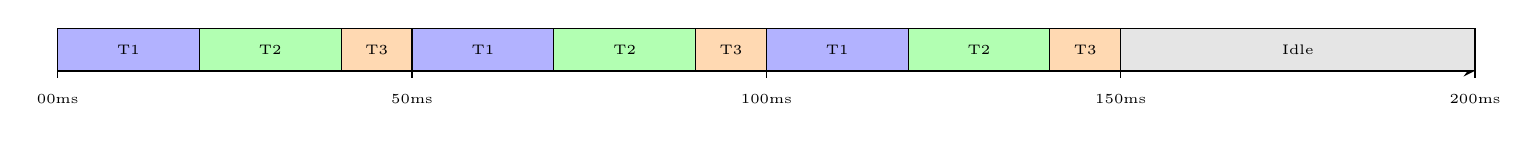
\begin{tikzpicture}[
    scale=0.9,
    timeline/.style={thick, -stealth},
    task/.style={rectangle, draw, fill=blue!30, minimum width=1cm, minimum height=0.6cm, text centered, font=\tiny},
    idle/.style={rectangle, draw, fill=gray!20, minimum width=1cm, minimum height=0.6cm}
  ]
    % Timeline
    \draw[timeline] (0,0) -- (20,0);
    \foreach \x in {0,5,10,15,20} {
      \draw (\x, -0.1) -- (\x, 0.1);
      \node[below, font=\tiny] at (\x, -0.2) {\x0ms};
    }
    
    % Tasks
    \draw[fill=blue!30] (0, 0) rectangle (2, 0.6) node[midway, font=\tiny] {T1};
    \draw[fill=blue!30] (5, 0) rectangle (7, 0.6) node[midway, font=\tiny] {T1};
    \draw[fill=blue!30] (10, 0) rectangle (12, 0.6) node[midway, font=\tiny] {T1};
    
    \draw[fill=green!30] (2, 0) rectangle (4, 0.6) node[midway, font=\tiny] {T2};
    \draw[fill=green!30] (7, 0) rectangle (9, 0.6) node[midway, font=\tiny] {T2};
    \draw[fill=green!30] (12, 0) rectangle (14, 0.6) node[midway, font=\tiny] {T2};
    
    \draw[fill=orange!30] (4, 0) rectangle (5, 0.6) node[midway, font=\tiny] {T3};
    \draw[fill=orange!30] (9, 0) rectangle (10, 0.6) node[midway, font=\tiny] {T3};
    \draw[fill=orange!30] (14, 0) rectangle (15, 0.6) node[midway, font=\tiny] {T3};
    
    % Idle
    \draw[fill=gray!20] (15, 0) rectangle (20, 0.6) node[midway, font=\tiny] {Idle};
  \end{tikzpicture}
  \caption{Beispiel: Task-Scheduling-Diagramm (Fixed-Priority)}
  \label{fig:task_scheduling}
\end{figure}

\subsection{Netzwerk-Berechnungen}

\subsubsection{TSN-Latenz-Berechnung}

Die TSN-Latenz setzt sich zusammen aus:

\begin{equation}
L_{TSN} = L_{tx} + L_{sw} + L_{gate} + L_{queue}
\end{equation}

wobei:
\begin{itemize}
  \item $L_{tx}$: Übertragungslatenz
  \item $L_{sw}$: Switch-Verarbeitungslatenz
  \item $L_{gate}$: Gate-Latenz (abhängig vom Gate-Schedule)
  \item $L_{queue}$: Warteschlangenlatenz
\end{itemize}

\subsubsection{Netzwerk-Auslastung}

Die Netzwerk-Auslastung berechnet sich als:

\begin{equation}
U_{net} = \frac{\sum_{i=1}^{n} (S_i \times F_i)}{B}
\end{equation}

wobei:
\begin{itemize}
  \item $S_i$: Frame-Größe von Flow $i$
  \item $F_i$: Frequenz von Flow $i$
  \item $B$: Bandbreite des Links
\end{itemize}

\subsection{Energie-Berechnungen}

\subsubsection{Dynamischer Energieverbrauch}

Der dynamische Energieverbrauch:

\begin{equation}
E_{dyn} = \alpha \times C \times V_{dd}^2 \times f \times t
\end{equation}

wobei:
\begin{itemize}
  \item $\alpha$: Switching-Aktivität
  \item $C$: Kapazität
  \item $V_{dd}$: Versorgungsspannung
  \item $f$: Frequenz
  \item $t$: Zeit
\end{itemize}

\subsubsection{Statischer Energieverbrauch}

Der statische Energieverbrauch:

\begin{equation}
E_{stat} = V_{dd} \times I_{leak} \times t
\end{equation}

wobei $I_{leak}$ der Leckstrom ist.

\section{Erweiterte Tabellen: Performance-Benchmarks}

Dieser Abschnitt enthält Performance-Benchmarks für verschiedene Komponenten.

\subsection{CPU-Performance-Benchmarks}

\begin{table}[h]
  \centering
  \caption{CPU-Performance-Benchmarks}
  \begin{tabular}{lllll}
    \toprule
    CPU-Typ & Kerne & Frequenz & DMIPS & Anwendung \\
    \midrule
    ARM Cortex-A78 & 8 & 2.8 GHz & 35,000 & AD-DC \\
    ARM Cortex-A55 & 4 & 2.0 GHz & 8,000 & Zonen-Controller \\
    Intel Atom & 4 & 1.6 GHz & 12,000 & Infotainment \\
    \bottomrule
  \end{tabular}
  \label{tab:cpu_benchmarks}
\end{table}

\subsection{GPU-Performance-Benchmarks}

\begin{table}[h]
  \centering
  \caption{GPU-Performance-Benchmarks}
  \begin{tabular}{lllll}
    \toprule
    GPU-Typ & TFLOPS & TOPS & Anwendung \\
    \midrule
    NVIDIA DRIVE Thor & 2000 & 2000 & AD-DC \\
    Qualcomm Snapdragon & 200 & 200 & Infotainment \\
    \bottomrule
  \end{tabular}
  \label{tab:gpu_benchmarks}
\end{table}

\section{Erweiterte Code-Beispiele}

Dieser Abschnitt enthält weitere Code-Beispiele für verschiedene Aspekte.

\subsection{Beispiel: Python-Transformations-Skript}

\begin{verbatim}
import json
from transformer import ArchitectureTransformer

# Load PREEvision export
with open('architecture.json', 'r') as f:
    arch_data = json.load(f)

# Create transformer
transformer = ArchitectureTransformer()

# Transform to OMNeT++
omnet_model = transformer.transform(
    arch_data,
    target_platform='omnetpp',
    config={
        'tsn_enabled': True,
        'redundancy_enabled': True
    }
)

# Save result
omnet_model.save('omnet_model.ned')
\end{verbatim}

\subsection{Beispiel: YAML-Mapping-Regel}

\begin{verbatim}
mapping_rules:
  - name: ECU_to_StandardHost
    source: ECU
    target: StandardHost
    attributes:
      cpu_cores: cpu_cores
      ram: ram_gb
      flash: flash_gb
    constraints:
      - cpu_cores > 0
      - ram > 0
\end{verbatim}

